\documentclass[a4paper,10pt,twocolumn,english]{article}
%---------------------------------------------------------
\usepackage{subcaption}
\usepackage{babel}
\usepackage[utf8]{inputenc}
\usepackage[T1]{fontenc}
\usepackage{hyperref}
\usepackage{graphicx}
% \usepackage[ruled,vlined,linesnumbered]{algorithm2e}
\usepackage{bm}
\usepackage{cite}
\usepackage{amsmath}
\usepackage{amsthm}
\usepackage{amsfonts}
%---------------------------------------------------------
\newcommand{\eref}[1]{(\ref{#1})}
%---------------------------------------------------------
\title{\textbf{Better Call LoRA}}

\author{
    \begin{tabular}{c c}
        Robert Trifan & Stefan Popa \\
    \end{tabular}\\[0.5em]
    \footnotesize University of Bucharest
}

\date{\empty}

\begin{document}
\maketitle
%---------------------------------------------------------
\begin{abstract}
Low-rank adaptation (LoRA) has become a lightweight alternative to full fine-tuning for large language models. In this work, we benchmark vanilla LoRA and four recent LoRA variants: swapped-init LoRA (A = 0, B $\sim \mathcal{U}(-0.01, 0.01)$), LoRA-XS ($A \cdot R \cdot B$ factorisation), LoRA+ (learning rate scaling, i.e. $\eta_A \neq \eta_B$) and PiSSA-initialised LoRA ($\text{SVD}(W)$ warm-start) on the TinyLlama-1.1 B backbone and the GLUE SST-2 sentiment-classification task.  All experiments were performed on a single RTX 2070 (8 GB), enforcing strict memory budgets. We report classification accuracy, macro-F1, wall-clock training time and peak GPU memory to highlight the trade-offs each variant offers under resource constrained conditions.
\end{abstract}
%---------------------------------------------------------
\section{Introduction}

Large language models (LLMs) have rapidly become the de facto standard for various natural language processing tasks, ranging from search and dialog to code generation and summarization. Their ubiquity is largely attributed to their capacity to learn from vast amounts of data, but this comes at a cost: the computational resources required for training and fine-tuning these models are substantial.

Training or fully fine-tuning these models typically implies billions of parameters, weeks of GPU time and significant energy consumption. Such costs are often out of reach for many practitioners, leading to a growing interest in more efficient alternatives.

Low-rank adaptation (LoRA) \cite{hu2021loralowrankadaptationlarge} tackles this challenge by injecting a pair of low-rank matrices into the weights of a pre-trained model and learning only those additional parameters while freezing the original model. Despite the simplicity of the approach, LoRA has matched or even surpassed the performance of full fine-tuning on many tasks, while reducing the memory footprint and training time by orders of magnitude.

Building on top of this idea, a growing literature has emerged, proposing improvements that modify the initialization, learning rates schedules or factorisation structure of the low-rank matrices hoping to further enhance the effectiveness of LoRA. While these extensions are promising, their practical impact remains unclear due to inconsistencies in experimental setups.

This survey offers a comprehensive overview of five LoRA variants, including the original LoRA, and benchmarks them on a sentiment classification task using the TinyLlama-1.1B model \cite{zhang2024tinyllamaopensourcesmalllanguage} and the GLUE SST-2 dataset \cite{wang2019gluemultitaskbenchmarkanalysis}. By standardizing the model size, dataset and evaluation metrics, we aim to provide an apples-to-apples comparison of these methods under realistic resource constraints.

\section{Setup}

\subsection{Model}

We employ the \href{https://huggingface.co/TinyLlama/TinyLlama-1.1B-Chat-v1.0}{\texttt{TinyLLaMA-1.1B-Chat-v1.0}} model from HuggingFace, a 1.1B parameter decoder-only transformer trained on 3T tokens. The architecture features 22 layers, 32 attention heads and an embedding size of 2048. The dataset used during pretraining consists of 950B tokens from a mixture of \href{https://huggingface.co/datasets/cerebras/SlimPajama-627B}{Slimpajama} (excluding GitHub) and \href{https://huggingface.co/datasets/bigcode/starcoderdata}{Starcoderdata} (code only), with a natural language to code ratio of 7:3. Total training spanned 1.43M steps (just over 3 epochs). The model's scale relative to downstream datasets like SST-2 motivates low-rank fine-tuning approaches.

\subsection{Dataset}

The General Language Understanding Evaluation (GLUE) benchmark is a collection of diverse natural language understanding tasks designed to evaluate and compare the performance of language models across multiple domains. For downstream evaluation and fine-tuning, we use the Stanford Sentiment Treebank v2 (SST-2) from GLUE. SST-2 is a binary sentiment classification task over natural language movie reviews, for example:

\begin{itemize}
    \item \textbf{Sentence:} ``klein, charming in comedies like american pie and dead-on in election''
    \item \textbf{Label:} positive
\end{itemize}

The dataset contains 70,042 samples in total: 67,349 in the train set, 872 in the validation set, and 1,821 in the test set (labels hidden). From this, we use 20,000 samples for training and the full validation set of 872 samples. The total number of tokens in the training set is 760,459, which is kept consistent across all runs.

As per the label distribution, the training set is slightly asymmetrical, as it contains 8,940 negative samples and 11,060 positive samples. In contrast, the validation label distribution is nearly balanced, with 428 negative and 444 positive sentences.

\subsection{Training} During training, we cast SST-2 as a single-turn instruction-following language-model task. Formally, for every sentence \textit{sentence} and label \textit{sentiment}, we build the prompt \texttt{Classify the sentiment of this sentence: <sentence>\textbackslash n\textbackslash n.Sentiment: <sentiment>\textbackslash n}. The tokenized prompt is fed to the model as both \texttt{input\_ids} and \texttt{labels} to ensure the model learns to predict the sentiment label directly. All pretrained model weights stay frozen by setting \texttt{requires\_grad=False}, while the LoRA parameters are trained with a batch size of 1 and gradient accumulation of 16. Given TinyLLaMA's 1.1B parameters, the dataset is orders of magnitude smaller, both in tokens and examples. As such, we fine-tuned for a single epoch, since training beyond that risks overfitting.

\subsection{Evaluation} At validation time, we feed the same prompt \emph{without} the sentiment token \texttt{Classify the sentiment of this sentence: <sentence>\textbackslash n\textbackslash n.Sentiment:}. A single forward pass yields the logits for the final position. We verified that each label corresponds to a single token (e.g., " positive" and " negative") to ensure a valid head-to-head comparison in the final logit vector. We manually extract the token for each sentiment and look up its index in the model's vocabulary. The prediction is the index of the sentiment token with the highest logit.

\subsection{Metrics}
We evaluate each method using classification accuracy, macro F1-score, wall-clock training time, and peak GPU memory usage. Accuracy measures the proportion of correctly predicted sentiment labels, while macro F1-score does assumes class balance, which is compatible with the evaluation distribution presented above. We use Weights \& Biases (\href{https://wandb.ai/site/}{wandb}) to log all metrics in real time during training. Models are trained for 1250 steps with an evaluation round every 50 steps to monitor progression. Training time and peak GPU usage are measured from the beginning of the first step until the end of the last step, excluding model/tokenizer loading and initialization.


\subsection{Hardware} All experiments were run on a single NVIDIA RTX 2070 with 8 GB of GPU memory. We enforced strict memory budgets to ensure that all methods could be compared under the same conditions. The training time was measured in wall-clock time, and the peak GPU memory usage was monitored throughout the training process.

\section{Low Rank Adaptation}

\noindent\textbf{LoRA.}  Low-Rank Adaptation (LoRA) \cite{hu2021loralowrankadaptationlarge} freezes the pre-trained weight matrix $W\!\in\!\mathbb{R}^{d_{\text{out}}\times d_{\text{in}}}$ and learns a low-rank residual $\Delta W = B A$ with $A\!\in\!\mathbb{R}^{r \times d_{\text{in}}}$ and $B\!\in\!\mathbb{R} ^ {d_{\text{out}} \times r}$, rank $r\!\ll\!\min(d_{\text{out}},d_{\text{in}})$.  During fine-tuning the forward pass uses $W+\Delta W$ while gradients flow only through $A$ and $B$, reducing trainable parameters from $d_{\text{out}}d_{\text{in}}$ to $r(d_{\text{out}}+d_{\text{in}})$.  Because the base weights never change, LoRA brings large memory savings by orders of magnitude (no optimizer states on $W$) and enables faster experimentation on consumer GPUs.

\noindent\textbf{Swapped-init LoRA (A = 0, B $\sim\mathcal{U}$).}  The original LoRA initialises $A$ from a small normal distribution and sets $B$ to zero so that $\Delta W$ starts at 0.  Hayou~et~al.\ \cite{hayou2024impactinitializationlorafinetuning} dive deeper into the intuition behind this choice, arguing that it's is indeed better to start from (A = 0, B $\sim\mathcal{U}$) instead of (A $\sim\mathcal{N}$, B = 0) and the reason behind this might be that the first initialization allows the use of larger learning rates (without causing output instability) resulting in more efficient learning.

\noindent\textbf{LoRA-XS.} LoRA-XS \cite{balazy2024loraxslowrankadaptationextremely} adds an intermediate low-rank matrix $R\!\in\!\mathbb{R}^{r\times r}$ and factorises the residual as $\Delta W = A R B^{\top}$.  The extra $r^{2}$ parameters increase expressiveness while preserving the $\mathcal{O}(r(d_{\text{out}}+d_{\text{in}}))$ memory budget (for typical $r\!\ll\!d$ the $r^{2}$ term is negligible). Empirically, LoRA-XS allows for more expressive low-rank representations while maintaining the same memory footprint as vanilla LoRA.

\noindent\textbf{LoRA+}\cite{hayou2024loraefficientlowrank} modifies the original LoRA method by applying different learning rates to the low-rank matrices $A$ and $B$. Since $A\!\in\!\mathbb{R}^{r \times d_{\text{in}}}$ and $B\!\in\!\mathbb{R}^{d_\text{out} \times r}$ have completely different shapes, the authors argue that their differing dimensionality and roles justify independent optimization dynamics. Empirically, using a higher learning rate for $B$ (typically by a factor of 2-4 for LLaMA models) improves convergence and downstream performance.

\noindent\textbf{PiSSA.} PiSSA\cite{meng2025pissaprincipalsingularvalues} (Principal Singular Values and Singular Vectors Adaptation of Large Language Models) introduces a singular value decomposition (SVD)-based initialization strategy for LoRA. Given a target weight matrix \( W \in \mathbb{R}^{d_{\text{out}} \times d_{\text{in}}} \), PiSSA computes its SVD: \( W = U \Sigma V^\top \). The top-\( r \) singular components are then used to initialize the low-rank adaptation matrices \( A \) and \( B \) such that \( \Delta W = A B \), where \( A = U_{[:, :r]} \Sigma^{1 / 2}_{[:r, :r]} \in \mathbb{R}^{d_{\text{out}} \times r} \) and \( B = \Sigma^{1 / 2}_{[:r, :r]} V^\top_{[:, :r]} \). Furthermore, before freezing, the original weight matrix $W$ is replaced with the rest of the singular components, i.e., \( W = U_{[:, r:]} \Sigma_{[r:, r:]} V^\top_{[:, r:]} \in \mathbb{R}^{m \times n} \). By $\Sigma^{1 / 2}$ we mean the square root of the diagonal matrix $\Sigma$ and the slicing notations are consistent with PyTorch's tensor indexing. This initialization aligns the low-rank structure with the principal subspace of the original weight matrix, improving convergence speed and performance stability in downstream tasks. The notation used in this paper is the other way around compared to the original paper, i.e., $W = A B$ instead of $W = B A$.


%---------------------------------------------------------
\section{Experiments}

\subsection{LoRA variants}

We begin by comparing the original LoRA initialisation ($A \sim \mathcal{U}(-0.01, 0.01), B = 0$) with the swapped LoRA initialisation ($A = 0$, $B \sim \mathcal{U}(-0.01, 0.01)$) and with the LoRA-XS method, ($A \sim \mathcal{U}(-0.01, 0.01), B = 0, R = I_r$, with $I_r$ being the identity matrix). All three methods use five different ranks: 2, 4, 8, 16, and 32. Additionally, we tested with $\alpha = 16$ and a learning rate of $2 \times 10 ^ {-4}$. The results presented in Figure~\ref{fig:ba_init} show that the swapped LoRA initialisation outperforms the original LoRA initialisation in most cases. However, both initialisation schemes are surpassed by the LoRA-XS method for all ranks, which is explained by the additional expresivity introduced by the intermediate low-rank matrix $R$. Results show as well that performance increases with the rank, achieving the peak for ranks 8 and 16, and diminishing afterwards.

\begin{figure}[ht]
    \centering
    \includegraphics[width=1\linewidth]{../plots/ba_init_eval_acc_f1_heatmaps.pdf}
    \caption{Accuracy and F1-score comparison between three different LoRA initialisations: original (A $\sim \mathcal{U}(-0.01, 0.01)$, B = 0), swapped-\texttt{init} (A = 0, B $\sim \mathcal{U}(-0.01, 0.01)$), and LoRA-XS (A $\sim \mathcal{U}(-0.01, 0.01)$, B $\sim \mathcal{U}(-0.01, 0.01)$).}
    \label{fig:ba_init}
\end{figure}



\subsection{LoRA+}

We used the official implementation of LoRA+ which can be found at the GitHub repository \href{https://github.com/nikhil-ghosh-berkeley/loraplus}{nikhil-ghosh-berkeley/loraplus}. Following the paper, we tested with $\alpha = 16$ and $r = 32$. For the learning rates we leveraged a grid-search over the following values: $\eta_A \in \{10^{-5}, 5 \times 10^{-5}, 10^{-4}\}$ and $\eta_B \in \{10^{-4}, 2 \times 10^{-4}, 4 \times 10^{-4}\}$. Results presented in Figure~\ref{fig:lora_plus} show that the best performing ratio $\eta_B / \eta_A$ is 4, with $\eta_A = 10^{-4}$. Picking the right learning rates is still crucial, but using a different learning rate for $B$ not only yields better results, but also allows for faster convergence. A very interesting observation is that configurations with same value of $\eta_A \cdot \eta_B$ have similar convergence speed.

\begin{figure}[ht]
    \centering
    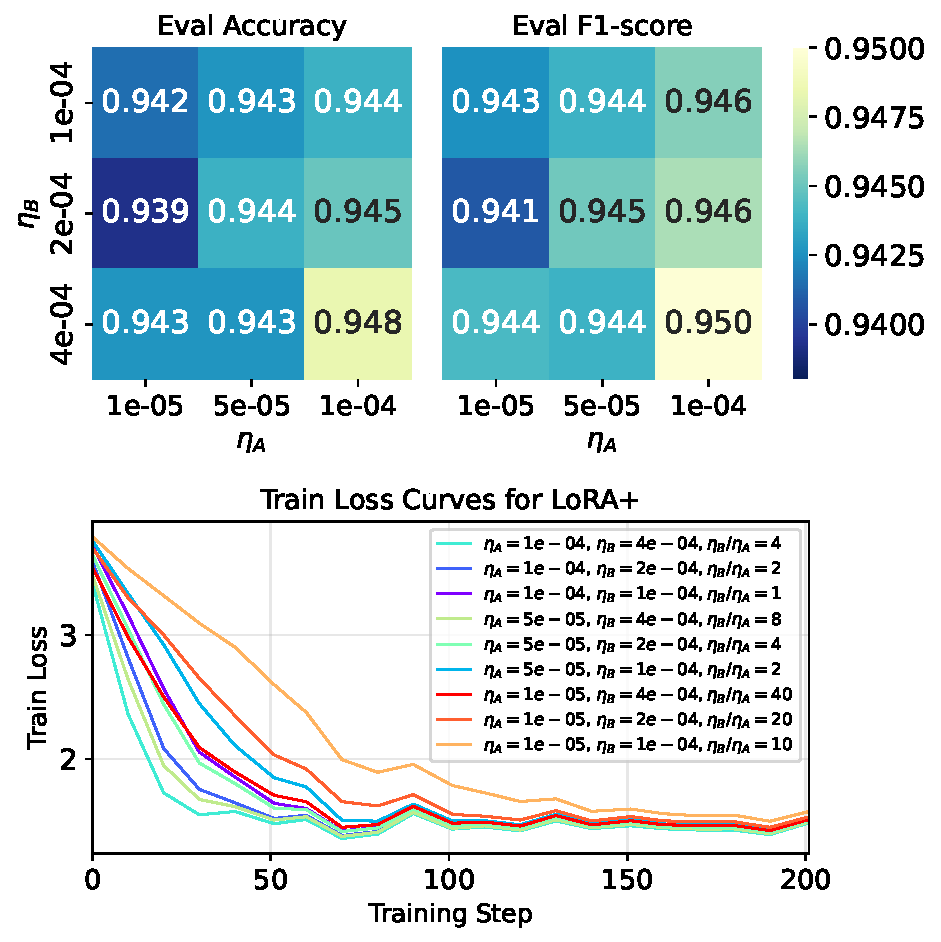
\includegraphics[width=1\linewidth]{../plots/lora_plus_train_loss_curves_final_v2.pdf}
    \caption{Accuracy and F1-score for LoRA+ with different learning rates for $A$ and $B$. Only the first 200 out of 1250 steps are shown for clarity.}
    \label{fig:lora_plus}
\end{figure}

\subsection{PiSSA}

Since PiSSA is integrated with \href{https://github.com/huggingface/peft}{PEFT}, we used the implementation provided by this library. For these experiments we used a learning rate of $5 \times 10^{-5}$ and three rank values: 2, 4, and 8. As in the PiSSA paper, we used $\alpha = r$. The results presented in Figure~\ref{fig:pissa} denote that performance and convergence speed increase with the rank, which is expected as the low-rank matrices capture more information from the original weight matrix. However, with larger increases in rank the GPU consumption follows the same trend, and the performance gains are marginal.

\begin{figure}[ht]
    \centering
    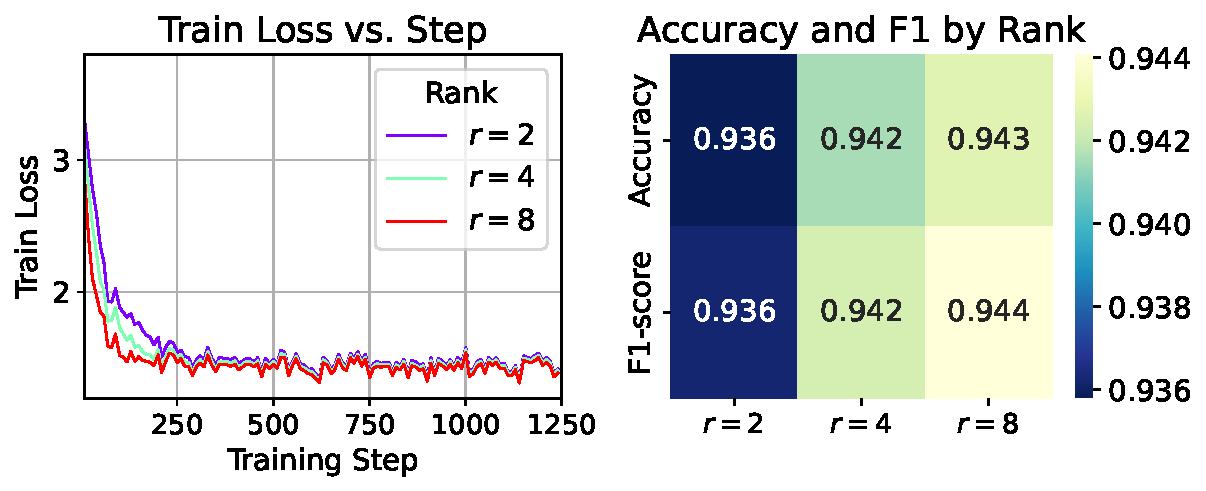
\includegraphics[width=1\linewidth]{../plots/pissa_train_loss_vs_step_final_v3.pdf}
    \caption{On the left side, training loss for PiSSA finetuning with different ranks. On the right side, accuracy and F1-score for the same runs.}
    \label{fig:pissa}
\end{figure}

%---------------------------------------------------------
\section{Conclusion}
Explain that, because of limited compute resources, we couldn't see meaningful results.

\bibliography{mybib}
\bibliographystyle{plain}

\end{document}
